\RequirePackage{snapshot}
\RequirePackage[final]{graphicx}
\documentclass[twocolumn,draft,aps,nofootinbib,nobibnotes,final]{revtex4-2}

% revtex4 imports the natbib package which conflicts with biblatex. To remedy the resulting name conflicts the following recipe is taken from https://tex.stackexchange.com/a/37077
% Start of 'ignore natbib' hack
%\let\bibhang\relax
%\let\citename\relax
%\let\bibfont\relax
%\let\Citeauthor\relax
%\let\textcite\relax
%\makeatletter
%\DeclareRobustCommand{\MakeUppercase}[1]{{%
%      \def\i{I}\def\j{J}%
%      \def\reserved@a##1##2{\let##1##2\reserved@a}%
%      \expandafter\reserved@a\@uclclist\reserved@b{\reserved@b\@gobble}%
%      \protected@edef\reserved@a{\uppercase{#1}}%
%      \reserved@a
%   }}
%\DeclareRobustCommand{\MakeLowercase}[1]{{%
%      \def\reserved@a##1##2{\let##2##1\reserved@a}%
%      \expandafter\reserved@a\@uclclist\reserved@b{\reserved@b\@gobble}%
%      \protected@edef\reserved@a{\lowercase{#1}}%
%      \reserved@a
%   }}
%\makeatother
%\expandafter\let\csname ver@natbib.sty\endcsname\relax
% End of 'ignore natbib' hack

%\usepackage{graphicx}

% For highlighting differences between original and revised versions
% Note (following https://tex.stackexchange.com/a/23308/2064) when highlighting text using \hl{} command
% we have to enclose any \ref{} or \cite{} or similar commands in extra curly brackets \ref{} -> {\ref{}}.
%\usepackage{soul}

\usepackage{amsmath,amssymb,amsfonts,amsthm}
%\usepackage[sort&compress,numbers]{natbib}
%\usepackage[english]{babel}

\usepackage{enumerate}
\usepackage{enumitem}
\usepackage{epsfig}
\usepackage{latexsym}
\usepackage{xcolor}
\usepackage[colorinlistoftodos, shadow, textsize=small]{todonotes}

\usepackage[colorlinks=true,citecolor=blue,linkcolor=blue,final]{hyperref}
%\usepackage{hyperref}

%\usepackage{hypernat}

\usepackage{comment}

% Jan 4, 2023: Added package multirow for multirow table
\usepackage{multirow}

% Biblatex setup
% The default is the 'numerical' style.
%\usepackage[backend=biber,url=true,eprint=true,doi=true,sorting=none,backref=true,style=phys]{biblatex}
% We use the following bibliography databases:
%\usepackage{bibtex}
%\addbibresource{../bib_library.bib}
% End biblatex


%%% BEGIN Custom commands %%%
\newcommand{\bite}{\begin{itemize}}
	\newcommand{\eat}{\end{itemize}}
\newcommand{\beq}{\begin{equation}}
	\newcommand{\eeq}{\end{equation}}
\newcommand{\rarrow}{\rightarrow}
\newcommand{\beqa}{\begin{align}}
	\newcommand{\eeqa}{\end{align}}
\newcommand{\barr}{\begin{array}}
	\newcommand{\earr}{\end{array}}
\newcommand{\del}{\partial}
\newcommand{\de}{\mathrm{d}}
%\newcommand{\mu\nu}{{\mu\nu}}
\renewcommand{\th}{\mathrm{th}}
\newcommand{\com}[1]{\begin{itemize}\color{RED}{{#1}}\end{itemize}}
\newcommand{\C}{\mathbb{C}}
\newcommand{\R}{\mathbb{R}}
\newcommand{\btw}[1]{\color{PURPLE}{{#1}}\color{BLACK}}
\newcommand{\cut}[1]{\color{RED}{{#1}}\color{BLACK}}

%text
\newcommand{\ie}{\textit{i.e.}~}
\newcommand{\eg}{\textit{e.g.}~}
\newcommand{\wrt}{\textit{w.r.t.}~}
\newcommand{\etc}{\textit{etc.}~}


\newcommand{\M}{\mathcal{M}}
\newcommand{\N}{\mathcal{N}}
% \newcommand{\H}{\mathcal{H}}

\newcommand{\bz}{\mathbf{z}}

\newcommand{\mb}[1]{\mathbf{#1}}
\newcommand{\mc}[1]{\mathcal{#1}}
\newcommand{\mbb}[1]{\mathbb{#1}}
\newcommand{\mf}[1]{\mathfrak{#1}}

\newcommand{\unit}[1]{\mathbf{\hat{#1}}}

%% Package bbold for bold identity symbol
\usepackage{bbold}

\newcommand{\id}{\mathbb{1}}

\newcommand{\utilde}[1]{\underaccent{\tilde}{#1}}

\newcommand{\vect}[1]{\boldsymbol{#1}}
\newcommand{\bvec}[1]{\boldsymbol{\vec #1}}
\newcommand{\expect}[1]{\langle #1\rangle}
\newcommand{\innerp}[2]{\langle #1 \vert #2 \rangle}
\newcommand{\expectop}[3]{\langle #1 \vert #2 \vert #3 \rangle}
\newcommand{\bra}[1]{\langle #1 \vert}
\newcommand{\ket}[1]{\vert #1 \rangle}
\newcommand{\supersc}[1]{$^{\textrm{#1}}$}
\newcommand{\subsc}[1]{$_{\textrm{#1}}$}
\newcommand{\sltwoc}{\mathfrak{sl}(2,\mathbb{C})}

\newcommand{\norm}[1]{\lVert #1 \rVert}

\newcommand{\rket}[1]{\vert #1 ]}
\newcommand{\rbra}[1]{[ #1 \vert}

\newcommand{\rinnerp}[2]{[ #1 \vert #2 ]}

\newcommand{\bket}[1]{\vert #1 )}
\newcommand{\bbra}[1]{( #1 \vert}

\newcommand{\binnerp}[2]{( #1 \vert #2 )}

\newcommand{\innerpA}[2]{\langle #1 \vert #2 ]}
\newcommand{\innerpB}[2]{[ #1 \vert #2 \rangle}

\newcommand{\onehalf}{\frac{1}{2}}

\newcommand{\Tr}{\mathrm{Tr}}

\newcommand{\Cyl}{\mathrm{Cyl}}
%%% END Custom commands %%%

\graphicspath{{figures/}}

%opening
\begin{document}

\preprint{This line only printed with preprint option}

\title{Thermal Intertwiners}

\author{Deepak Vaid}
\email{dvaid79@gmail.com}
\affiliation{}
\author{Sumukha Srinivasa Adiga}
\email{sumukha.s.adiga@gmail.com}
\affiliation{}

\date{\today}

\begin{abstract}
Constructing semiclassical states of quantum geometry which resemble a smooth macroscopic Riemannian geometry on large enough scales continues to remain a challenge. Moreover in any theory of quantum gravity one should be able to provide a description of geometric states which correspond to systems at finite temperature. This would have implications, for instance, for the description of black hole horizons in quantum gravity. In loop quantum gravity, $ U(N) $ coherent states (coherent intertwiners) provide one avenue towards constructing such states. In this work we show that the structure of these coherent intertwiners allows one to make contact with a thermal description of states of quantum geometry \textit{without needing to introduce any extra ingredients into the picture}. We show how to define, via a Boguliubov transformation, thermal states for each face of such an intertwiner. We then argue that asking such faces to be glued to one other implies the presence of thermal equilibrium between different faces and an equipartition property for thermal intertwiners.
\end{abstract}

\maketitle

\tableofcontents

\listoftodos

\section{Introduction}

Quantum geometry must necessarily be an integral part of any theory of quantum gravity. By ``quantum geometry'' we refer to the structures which replace classical geometric concepts of lines, surfaces and volumes at the Planck scale. There is ample evidence to suggest that the spacetime which we perceive as a smooth manifold on nearly all scales, from subatomic to cosmological, must give way to a discrete, fluctuating geometric ``foam'' at the Planck scale. It is natural to expect that this quantum ``foam'' must have a quantum mechanical description and consistency requires that at sufficiently large scales the quantum mechanical description should begin to coincide with the classical picture of a smooth manifold. In quantum mechanics such states whose description is \textit{as close as possible} to classical states are known as coherent states.

A second essential aspect of any picture of quantum geometry should be a concept of thermal states which correspond to fluctuating geometries. It is by now standard lore that gravity and thermodynamics are inextricably intertwined. Half a century ago, Bekenstein realized that black holes should be thermal objects which possess an entropy and a temperature. It was realized soon after by Hawking, Carter, Bardeen and others a black hole should radiate at a temperature proportional to the surface gravity of its horizon and that black holes should obey a set of laws of black hole thermodynamics in complete analogy with ordinary thermal systems. One might even go so far as to argue, following Jacobson \todo{reference}, Padmanabhan \todo{reference} and Verlinde \todo{reference}, that Einstein's field equations are a consequence of imposing local thermal equilibrium between the degrees of freedom of geometry and matter. These developments suggest that in any theory of quantum gravity it should be possible to construct thermal states of quantum geometry.

Combining the above two insights implies that any theory of quantum gravity must permit the construction of \textit{thermal coherent states} of quantum geometry.

One framework which permits the construction of such a quantum geometry is loop quantum gravity (LQG). In LQG there exist several candidate constructions of coherent states of geometry which are \textit{peaked} around classical geometries with given values of geometric parameters such as the amount of intrinsic and extrinsic curvature of a surface. The construction of thermal states in LQG, however, has not been as successful as the coherent state program. In particular it would be desirable to be able to construct thermal coherent states of spin networks which correspond to semiclassical geometries at non-zero temperature. Some progress has been made towards this goal in the Group Field Theory (GFT) program \todo{reference to Kotecha et al}, which can be viewed a second quantization of LQG.

The layout of this work is as follows. In \autoref{sec:u-n-coherent-states} we review the construction of the classical phase space the and quantum state space for a single $ N $-valent vertex, which could be part of a larger spin network, and recall how the degrees of freedom living on the faces of the polyhedron can be described using two independent harmonic oscillators. We then describe the construction of the spinorial version of the classical LQG phase space. This will be useful in the construction of coherent states in the following sections. In \autoref{sec:thermal-coherent-states} we explain how one can construct thermal states and coherent states for a single harmonic oscillator and how the two notions can be combined to give us thermal coherent states - i.e. states which obey the coherence property required for them to approximate classical behavior and also possess thermal properties parameterized by a temperature. In \autoref{sec:u-n-thermal-coherent-states} we begin by reviewing the construction of $ U(N) $ coherent intertwiners which correspond to semiclassical states of polyhedral geometries. We then point out that the Schwinger boson representation which is utilized in constructing these states has all the necessary ingredients required to construct thermal states for each face of a polyhedron by performing a simple Boguliubov transformation on the face variables. The Boguliubov transformation depends on a parameter $ \theta $ which can be identified with the temperature of the state. \textit{A priori} there is no reason to take $ \theta $ to be the same of all faces of the polyhedron. However, we argue that if this is not the case it becomes problematic to identify the resulting geometry with a semiclassical polyhedron which satisfies the closure condition on face normals. If we generalize from polyhedra to arbitrary two dimensional surfaces constructed by gluing quanta of area together then this line of reasoning suggests that such states represent semiclassical states of geometry only when the temperature parameter is the same for each area quantum, implying the requirement of a thermal equipartition property on semiclassical states of quantum geometry. We conclude with discussion of these results and some speculations.

\section{Thermal coherent states}\label{sec:thermal-coherent-states}

\subsection{Coherent states}\label{sec:coherent-states}

Coherent states are the semi-classical states of quantum theory. The coherent state minimizes the uncertainty relation by minimizing and equating both $\Delta x$ and $\Delta p$. The coherent states $ \ket{\alpha} $ of a harmonic oscillator are eigenvectors of the annihilation operator:
\begin{align}
	a \ket{\alpha} = \alpha \ket{\alpha} 
\end{align}

The state $\ket{\alpha}$ can also be created by acting with the displacement operator $ D(\alpha) $ on the ground state:
\begin{align}\label{eqn:coherent-state-transform}
	\ket{\alpha} &= D(\alpha)\ket{0}
\end{align}
where the displacement operator $D(\alpha)$ is given by 
\begin{align}\label{eqn:displacement-operator}
	D(\alpha) &= \exp(\alpha a^{\dagger} - \alpha^{*}a)
\end{align}
The coherent state $\ket{\alpha}$ can be expressed as a superposition of the energy eigenstates and it is given as : 
\begin{align}\label{eqn:coherent-state-expr}
	\ket{\alpha} = e^{-\frac{|\alpha|^2}{2}} \sum_{n=0}^{n=\infty} \frac{\alpha^{n}}{\sqrt{n!}}\ket{n}
\end{align}
What makes these states so special is the fact that the real and imaginary components of the parameter $ \alpha $ can be interpreted as the position and momentum of a \textit{classical} harmonic oscillator as shown in \autoref{fig:sho-phase-space}.
\begin{figure}
	\centering
	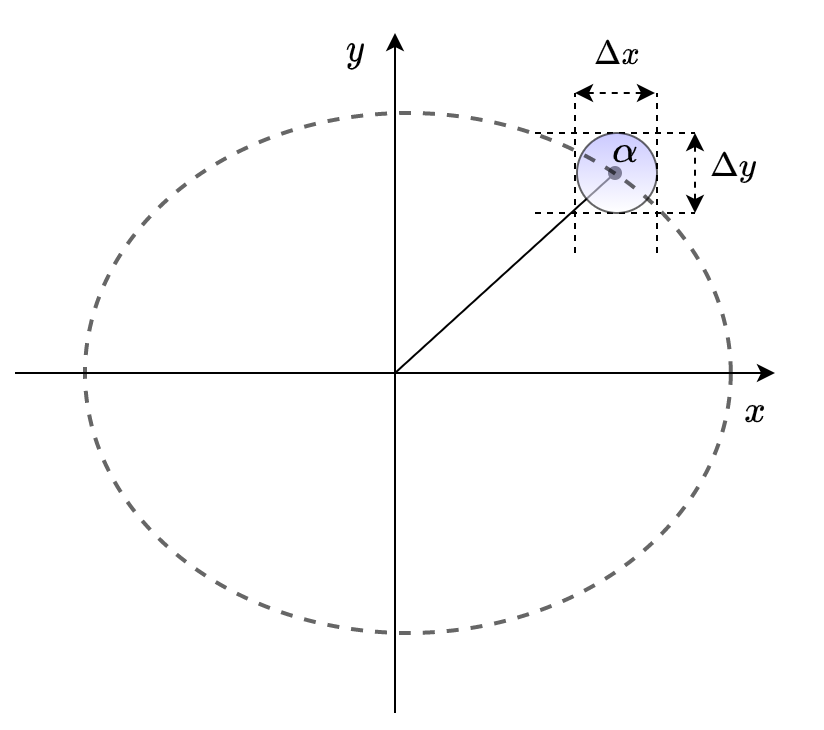
\includegraphics[width=0.7\linewidth]{figures/sho-phase-space}
	\caption{The parameter $ \alpha $ which labels the coherent state $ \ket{\alpha} $ encodes the phase space co-ordinates of an ordinary classical oscillator. Time-evolution of the coherent state under the Schrödinger Hamiltonian yields a trajectory for $ \alpha $ which is precisely that of the classical oscillator.}
	\label{fig:sho-phase-space}
\end{figure}
Moreover under time evolution coherent states remain coherent, \ie the property of classicality of a coherent state is maintained over time. It would not be sufficient to have states which were ``coherent'' (saturated the uncertainty bound) at a single time if time-evolution would cause that coherence to dissipate.

In addition to the property of coherence, as described above, we would like to endow our states with a thermodynamic description. It is well known how to construct ``thermal states'' in many body quantum mechanics and in quantum field theory. Is it possible to construct thermal states of quantum geometry which are also coherent? This would correspond to quantum states which describe the behavior of semi-classical geometries at finite temperature. Examples of such systems are the apparent horizon seen by an observer in a Rindler spacetime, or the ``real'' horizon seen by a static observer located outside a Schwarzschild black hole. To make progress towards this stage we first discuss the construction of thermal states and then thermal coherent states in the following two subsections.

\subsection{Thermofield Double States}\label{sec:tfd-state}

Traditionally there are two principle methods \cite{Khanna2009Thermal} which are used to construct thermal ensembles in quantum theory. The first method rests upon the notion of a density matrix $ \rho $ which describes the state of a system at a given time. The condition of thermal equilibrium is imposed quantitatively by the following two constraints on $ \rho $. These are:
\begin{enumerate}[label=\emph{\alph*})]
	\item \textbf{Time independence:} The thermal state should be time-independent:
	\begin{equation}\label{eqn:thermal-condition-1}
		i\frac{\partial \rho(t)}{\partial t} = [\hat H, \rho(t)] = 0
	\end{equation}
	\item \textbf{Entropy maximization (Second law):} When the system is in thermal equilibrium, small variations in the state should not change the entropy of the system:
	\begin{equation}\label{eqn:entropy-maximization}
		\delta S[\rho] = 0
	\end{equation}
\end{enumerate}
With these two assumptions in hand one can show \cite{Khanna2009Thermal} that at thermal equilibrium the density matrix of a system, in the canonical ensemble, is by the following expression:
\begin{equation}\label{eqn:thermal-density-matrix}
	\rho(\beta) =  \frac{1}{Z}\exp{(-\beta \hat H)},
\end{equation}
where $ Z = \Tr[\exp(-\beta \hat H)] $ is a normalization constant which we also recognize to be the partition function of the system. Here $ \hat H $ is the Hamiltonian of the system and $ \beta = (k_B T)^{-1} $ is the inverse temperature in Boltzmann units. Given any observable $ \hat A $ the corresponding thermal expectation value is given by:
\begin{equation}\label{eqn:thermal-expectation-value-1}
	\expect{\hat A} = \Tr[ \rho \hat A]
\end{equation}
In analogy with the Gibbsian description of classical thermal equilibrium one can write down an expression for the entropy of a system described by a density matrix $ \rho $:
\begin{equation}\label{eqn:von-neumann-entropy}
	S_{vN} = - k_B \Tr[\rho \ln \rho]
\end{equation}
also known as the von-Neumann entropy.

The second approach, known as thermofield dynamics, starts by asking the question about whether or not it is possible to construct a state $ \ket{0(\beta)} $ which represents the thermal ground state of a given system, such that thermal expectation values of any observables can be obtained by taking the expectation of the associated operator in the thermal ground state:
\begin{equation}\label{eqn:thermal-expectation-value-2}
	\expect{\hat A} = \expectop{0(\beta)}{\hat A}{0(\beta)}
\end{equation}
Now, morally speaking, it might appear that is no real difference between \eqref{eqn:thermal-expectation-value-1} and \eqref{eqn:thermal-expectation-value-2} since for a pure state $ \rho = \ket{\psi}\bra{\psi} $ and the expression \eqref{eqn:thermal-expectation-value-1} reduces to \eqref{eqn:thermal-expectation-value-2} using the cyclic property of the trace:
\begin{equation*}
	\Tr[\rho \hat A] = \Tr[\ket{\psi}\bra{\psi} \hat A] = \bra{\psi} \hat A \ket{\psi}
\end{equation*}
However, there is a crucial difference due to the fact that the density matrix in \eqref{eqn:thermal-expectation-value-1} need not be that of a pure state, whereas in \eqref{eqn:thermal-expectation-value-2} we are requiring that the state $ \ket{0(\beta)} $ must be a pure state. It turns out the second construction is possible if one introduces a \emph{second} auxiliary Hilbert space which is a copy of the original system and the thermal state $ \ket{0(\beta)} $ then lives in the tensor product space. As shown by Takahashi and Umezawa \cite{Takahashi1996Thermo} we can define an extended Hilbert space:
\begin{align}
	\mc{H} = \mc{H}_{L}\otimes \mc{H}_{R}
\end{align}
where $\mc H_{L}$ and $ \mc H_{R}$ stand for the ordinary Hilbert spaces for the zero temperature theory on the left hand side and the right hand side, respectively. We define $a_{L} $ and $a_{L}^{\dagger}$ as the annihilation and creation operators acting on $ \mc H_L $ and likewise for $ \mc H_R $. These operators satisfy the commutation relation:
\begin{align}\label{eqn:ladder-ops}
	[a_{L},a_{L}^{\dagger}] &= [a_{R},a_{R}^{\dagger}] = 1 \\
	[a_{L},a_{R}] &= 0
\end{align}
Given the form of \eqref{eqn:thermal-expectation-value-2} it turns out to be fairly straightforward to show (see \autoref{sec:tfd}) that the state $ \ket{0(\beta)} $ can be written in terms of the energy eigenbasis of $ \mc H_L $ and $ \mc H_R $ as follows:
\begin{equation}\label{eqn:tfd-state}
	\ket{0(\beta)} = \frac{1}{\sqrt{Z(\beta)}} \sum_n e^{-\beta E_n /2} \ket{n, \tilde n},
\end{equation}
where $ \ket{n}, \ket{\tilde n} $ are eigenstates of the number operators $ a_L^\dagger a_L $ and $ a_R^\dagger a_R $ and in the expression above $ \tilde n = n $. The state $ \ket{0(\beta)} $ is also known as the ``thermo-field double'' (TFD) state. $ Z(\beta) $ is the partition function for the thermal state defined on a single copy of $ \mc H_0 $ \eqref{eqn:thermal-density-matrix}.

As explained in \autoref{sec:thermal-unitary} the state $ \ket{0(\beta)} $ can be obtained from the doubled oscillator vacuum $ \ket{0,\tilde 0} $ by the action of a unitary operator:
\begin{align}\label{eqn:thermal-ground-state}
	\ket{0(\beta)} = U(\beta)\ket{0}_{L}\ket{0}_{R}
\end{align}
The operator $U(\beta)$ is given by:
\begin{align}\label{eqn:u-beta}
	U(\beta) = \exp[\theta(a_{L}^{\dagger} a_{R}^{\dagger} - a_{L}a_{R})]
\end{align}
where $ \theta $ is related to $\beta$ by:
\begin{align}\label{eqn:theta-beta-relation}
	\cosh(\theta) &= (1-e^{-\beta w})^{-\frac{1}{2}} \\
	\sinh(\theta) &= (e^{\beta w} - 1)^{-\frac{1}{2}}
\end{align}
This transformation of states also induces a transformation of the creation and annihilation operators. The operator transformation is given by the Boguliubov transformation:
\begin{align}\label{eqn:thermal-ladder-ops}
	a_{L}(\beta) = U(\beta) a_{L} U^{\dagger}(\beta) &= \cosh(\theta) a_{L} - \sinh(\theta) a_{R}^{\dagger} \\
	a_{R}(\beta) = U(\beta) a_{R} U^{\dagger}(\beta) &= \cosh(\theta) a_{R} - \sinh(\theta) a_{L}^{\dagger}
\end{align}
With these ``thermal'' ladder operators on hand we can now construct thermal number operator states:
\begin{align}
	\ket{n_{1},n_{2}}_\beta = \frac{(a^{\dagger}_{L}(\beta))^{n_{1}}(a^{\dagger}_{R}(\beta))^{n_{2}}}{\sqrt{n_{1}!}\sqrt{n_{2}!}}\ket{0(\beta)}
\end{align}
The state \eqref{eqn:thermal-ground-state} has an important and interesting property which can be seen as follows. The exponential in \eqref{eqn:u-beta} when acting on the vacuum $ \ket{0}_L \ket{0}_R $ can be expressed as \cite{Guo2020Circuit}:
\begin{align}\label{eqn:thermal vacuum}
	U(\beta) \ket{0}_L \ket{0}_R & = \exp\left[\theta(a_{L}^{\dagger} a_{R}^{\dagger} - a_{L}a_{R})\right] \ket{0}_L \ket{0}_R \nonumber \\
	& = \frac{1}{\cosh(\theta)} \exp\left[\tanh(\theta) a^\dagger_L a^\dagger_R \right]\ket{0}_L \ket{0}_R \nonumber \\
	& = \frac{1}{\sqrt{1-e^{-\beta \hbar \omega}}} \sum_{n=0}^\infty e^{-n \beta \hbar \omega/2} \ket{n}_L \ket{n}_R \nonumber \\
\end{align}
In the limit of infinite temperature $ \beta \rarrow 0 $, the state $ \ket{0(\beta)} $ reduces to $ \sum_n \ket{n,n} $ which is (upto a normalization factor) the maximally entangled state in the doubled Hilbert space $ \mc H $. It is a remarkable fact that mixed thermal states in one Hilbert space can be mapped to highly entangled pure state in a doubled Hilbert space and this hints perhaps to the existence of a deeper connection between thermodynamics and entanglement.

\subsection{Thermal Coherent States}\label{sec:thermal-coherent-state-2}

We now have in hand the two ingredients we need to construct thermal coherent states. On the one hand we have the displacement operator \eqref{eqn:displacement-operator} which tells us how to construct a coherent state $ \ket{\alpha} $ labeled by a parameter $ \alpha $ \textit{given} a ground state $ \ket{0} $. On the other hand we have the ``thermalizing'' operator \eqref{eqn:u-beta} which takes the ground state of a doubled Hilbert space $ \ket{0,0} $ and converts it into a thermal ground state $ \ket{0(\beta)} $ as shown in \eqref{eqn:thermal-ground-state}. The way to create thermal coherent states is now seemingly clear. Create the thermal vacuum using the operator \eqref{eqn:u-beta} and \textit{then} act on the thermal vacuum with the displacement operator \eqref{eqn:displacement-operator} to obtain a thermal coherent state.

However, there is one minor issue. The coherent state construction requires only the original Hilbert space, whereas the thermal state construction requires a doubled Hilbert space. The solution to this problem is straightforward. We simply double the Hilbert space \textit{before} applying the coherent state transform. The thermal coherent state is then given by \cite{Guo2020Circuit} :
\begin{equation}\label{eqn:thermal-coherent-state}
	\ket{TC} = U(\beta) \ket{\alpha}_L \ket{\gamma}_R = U(\beta) D(\alpha, \gamma) \ket{0}_L \ket{0}_R,
\end{equation}
where the operator $ D(\alpha,\gamma) $ is now a displacement operator acting on the doubled Hilbert space and is simply given by the product of the the displacement operators on two copies of the original Hilbert space:
\begin{equation}\label{eqn:doubled-displacement}
	D(\alpha, \gamma) = D_L(\alpha) D_R(\gamma).
\end{equation}
Note that since we have two \textit{independent} coherent states we need two sets of the classical parameters $ \alpha $ and $ \gamma $.

There is a second route one can follow. Namely rather than constructing thermal coherent states $ \ket{TC} $, we construct coherent thermal states $ \ket{CT} $, \ie we first construct the thermal ladder operators $ a^\dagger(\beta) $ and $ a(\beta) $ \eqref{eqn:thermal-ladder-ops} using the operator $ U(\beta) $ and then construct coherent states using the displacement operator built with these thermalized ladder operators. These two approaches can be summarized as: displace then thermalize (for $ \ket{TC} $) or thermalize then displace (for $ \ket{CT} $). In what follows we will be using the latter approach to construct coherent thermal states for $ \mf{su}(2) $ using which one can immediately construct coherent thermal intertwiners.

\section{$ \mf{su}(2) $ Thermal Coherent States}\label{eqn:thermal-spin-state}

In this section we will show how one can construct thermal coherent states for a particle with a given spin $ j $. For this first we will review the Schwinger boson representation of the $ \mf{su}(2) $ algebra, following which we can use the procedure outlined in the previous section to construct thermal coherent states.

\subsection{Schwinger Boson Construction }\label{sec:schwinger-boson}

The Schwinger boson representation of the Hilbert space of a particle with spin $ j $ plays a central role in this work. We exploit the fact that one can express the Hilbert space of a \textit{single} spin $ j $ particle in terms of \textit{two} simple harmonic oscillators as follows. The $ \mf{su}(2) $ algebra is spanned by the operators $ J_x, J_y, J_z $. We introduce two sets of ladder operators $ a, a^\dag, b, b^\dag $ in terms of which the $ \mf{su}(2) $ operators can be expressed as follows:
\begin{equation}\label{eqn:schwinger-boson-rep}
	J_z = \onehalf (a^\dag a - b^\dag b); \quad J_+ = a^\dag b; \quad J_- = b^\dag a
\end{equation}
where $ J_{\pm} = J_x \pm i J_y $ are the usual angular momentum raising and lowering operators and $ a,a^\dag, b, b^\dag $ satisfy the familiar harmonic oscillator commutation relations:
\begin{equation}\label{eqn:sho-commutator}
	[a,a^\dag] = [b, b^\dag] = 1; \quad [a,b] =  [a, b^\dag] = 0
\end{equation}
It is easy to check that the operators \eqref{eqn:schwinger-boson-rep} defined in this way satisfy the usual $ \mf{su}(2) $ algebra: $ [J_i, J_j] = i \epsilon_{ijk} J_k $.

States in the Schwinger boson representation are given by acting on the harmonic oscillator Fock vacuum with the number operators for the two oscillators:
\begin{equation}\label{eqn:schwinger-states}
	\ket{n_a, n_b} = \frac{(a^\dag)^{n_a} (b^\dag)^{n_b}}{\sqrt{n_a ! n_b !}}\ket{0,0}
\end{equation}
The operator for the total energy of such a state is given by:
\begin{equation}\label{eqn:schwinger-energy-op}
	\mc{E} = \onehalf(a^\dag a + b^\dag b),
\end{equation}
with eigenvalues:
\begin{equation}\label{eqn:schwinger-energy-eigenvalues}
	\mc{E} \ket{n_a, n_b} = \onehalf (n_a + n_b) \ket{n_a, n_b}
\end{equation}
Similarly the eigenvalues of the $ J_z $ operator defined in \eqref{eqn:schwinger-boson-rep} are given by:
\begin{equation}\label{eqn:j-z-defn}
	J_z \ket{n_a, n_b} = \onehalf (n_a - n_b) \ket{n_a, n_b}
\end{equation}
This tells that we can identify $ n_a - n_b $ as the magnetic quantum number $ m $ for an angular momentum state $ \ket{j;m} $. Now by explicit calculation using \eqref{eqn:schwinger-boson-rep} and the definition of the energy operator \eqref{eqn:schwinger-energy-op} one can verify that:
\begin{equation}\label{eqn:j-square-defn}
	J^2 = \mc{E}(\mc{E}+1),
\end{equation}
where $ J^2 = J_x^2 + J_y^2 + J_z^2 $ is the $ \mf{su}(2) $ Casimir with eigenvalue $ j(j+1) $ when acting on the state $ \ket{j;m} $. This tells us that we can identify the eigenvalue of the energy operator $ \mc{E} $ with the angular momentum quantum number $ j $. So finally we see that the states of the harmonic oscillator space are in one-to-one correspondence with the usual angular momentum eigenbasis:
\begin{equation}\label{eqn:state-correspondence}
	\ket{j;m} \equiv \ket{n_a, n_b}; \quad j = \onehalf(n_a + n_b);~ m = \onehalf(n_a - n_b).
\end{equation}
In the next section we will see that $ j $  is a measure of the total area associated with an edge of a spin network, with the precise expression depending on which of the two prescriptions in \eqref{eqn:area-operators} is used for the area operator.

\begin{table}[]
	\begin{tabular}{|l|l|l|l|l|}
		\hline
		$ j $                    & $ m $    & $ n_a $ & $ n_b $ & $ \ket{n_a, n_b} $ \\ \hline
		\multirow{2}{*}{1/2} & +1/2 & 1   & 0   & $ \ket{1,0} $              \\ \cline{2-5} 
		& -1/2 & 0   & 1   & $ \ket{0,1} $              \\ \hline
		\multirow{3}{*}{1}   & +1   & 2   & 0   & $ \ket{2,0} $              \\ \cline{2-5} 
		& 0    & 1   & 1   & $ \ket{1,1} $              \\ \cline{2-5} 
		& -1   & 0   & 2   & $ \ket{1,0} $              \\ \hline
		\multirow{4}{*}{3/2} & +3/2 & 3   & 0   & $ \ket{3,0} $              \\ \cline{2-5} 
		& +1/2 & 2   & 1   & $ \ket{2,1} $              \\ \cline{2-5} 
		& -1/2 & 1   & 2   & $ \ket{1,2} $              \\ \cline{2-5} 
		& -3/2 & 0   & 3   & $ \ket{0,3} $              \\ \hline
	\end{tabular}
	\caption{Mapping between angular momentum states in the usual representation in terms of $ \ket{j;m} $ and states in the Schwinger boson representation $ \ket{n_a, n_b} $}
	\label{tbl:schwinger-boson-map}
\end{table}

The physical picture of the Schwinger boson states is the following. A single particle of spin $ j $ is described by a pair of free harmonic oscillators with the constraint that the \textit{total} energy $ \mc E $ of both oscillators is fixed and is related to given by $ j $ as seen in expressions \eqref{eqn:state-correspondence} and \eqref{eqn:schwinger-energy-eigenvalues}. The highest weight state $ \ket{j;j} $ with $ m = j $ corresponds to having one oscillator (say $ A $) at the highest energy ($ \mc E = j $) and the other (say $ B $) in the ground state. As we act on the spin with the spin lowering operator $ J_- $ we lower the energy of the $ A $ oscillator by one unit and increase the energy of the $ B $ oscillator by one unit. When we reach the lowest weight state $ \ket{j;-j} $ with $ m = -j $ the $ A $ oscillator is in the ground state while the $ B $ oscillator is in the highest energy $ \mc E $ state. This construction can be viewed as mapping a spin $ j $ system to a collection of $ 2j $ spin $ 1/2 $ particles with $ n_a $ spin up particles and $ n_b $ spin down particles as shown in \autoref{fig:schwinger-spins}.

\begin{figure}[htbp]
	\centering
	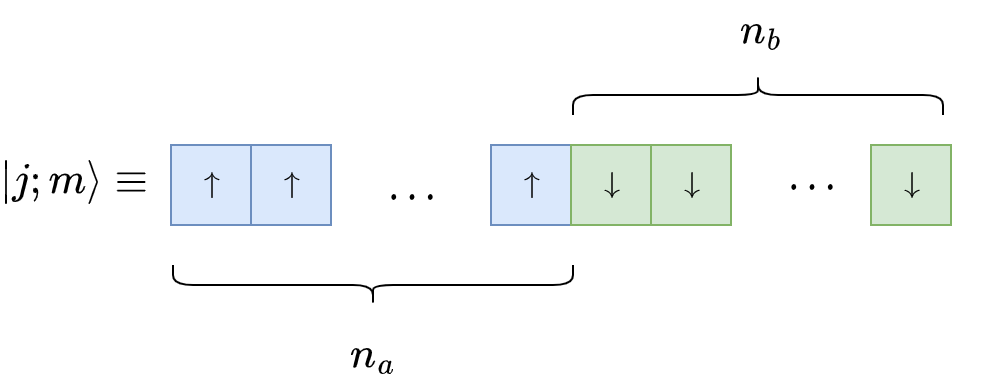
\includegraphics[width=0.9\linewidth]{schwinger-spins}
	\caption{Angular momentum state $ \ket{j;m} $ can be mapped to a system of $ 2j $ spin $ 1/2 $ particles.}
	\label{fig:schwinger-spins}
\end{figure}

\subsection{$ \mf{su}(2) $ Thermal Coherent State}\label{sec:su2-thermal-coherent-state}

Given the mapping between a pair of bosonic oscillators and the $ \mf{su}(2) $ algebra we can now put to use the techniques of the previous sections to construct thermal coherent states for a particle with spin $ j $. First let us remind ourselves how to construct coherent states for spin $ j $. Recall that the coherent state for a single oscillator is of the form given by \eqref{eqn:coherent-state-expr}. We can easily generalize this to build a coherent state for a \textit{pair} of oscillators. Following \cite[Appendix B]{Freidel2009The-Fine} we can write:
\begin{equation}\label{eqn:pair-coherent-state}
	\ket{z_a, z_b} = e^{-(|z_a|^2 + |z_b|^2)/2} \sum_{n_a, n_b} \frac{z_a^{n_a} z_b^{n_b}}{\sqrt{n_a! n_b!}} \ket{n_a, n_b},
\end{equation}
which is simply the tensor product of two copies of \eqref{eqn:coherent-state-expr} with parameters $ z_a $ and $ z_b $ respectively labeling the two coherent states and the state $ \ket{n_a, n_b} $ is given by \eqref{eqn:schwinger-states}. To obtain coherent states for a fixed spin $ j $ we simply need to project out those components which do not satisfy the constraint $ 2j = n_a + n_b $. If we write the projector as $ P_j $, then after a little bit of algebra (see \autoref{sec:spin-projection} for the details) one finds that:
\begin{equation}\label{eqn:spin-coherent-state}
	P_j \ket{z_a, z_b} = e^{-(|z_a|^2 + |z_b|^2)/2} z_a^{2j} \ket{j;z},
\end{equation}
where $ \ket{j;z} $ is given by:
\begin{equation}\label{eqn:su2-coherent-state}
	\ket{j;z} = \sum_{m=-j}^{j} \frac{z^{j-m}}{\sqrt{(j+m)! (j-m)!}} \ket{j;m},
\end{equation}
which is (upto normalization) the $ \mf{su}(2) $ coherent state. Using \eqref{eqn:schwinger-states} we can rewrite the above as:
\begin{equation}\label{eqn:su2-coherent-state-2}
	\ket{j;z} = \sum_{m=-j}^{j} \frac{z^{j-m} (a^\dagger)^{j+m} (b^\dagger)^{j-m}}{(j+m)! (j-m)!} \ket{0,0}
\end{equation}
Using this we can write down the expression for $ \mf{su}(2) $ thermal coherent states:
\begin{equation}\label{eqn:su2-thermal-coherent-state}
	\ket{z(\beta)} = \sum_{m=-j}^{j} \frac{z^{j-m} (a^\dagger(\beta))^{j+m} (b^\dagger(\beta))^{j-m}}{(j+m)! (j-m)!} \ket{0(\beta)},
\end{equation}
where $ a^\dagger(\beta), b^\dagger(\beta) $ are the thermalized ladder operators \eqref{eqn:thermal-ladder-ops} and $ \ket{0(\beta)} $ is the thermofield double ground state \eqref{eqn:tfd-state}.

%In order to do so we will proceed according to the second method described at the end of \autoref{sec:thermal-coherent-states}. First we will construct the thermal ground state $ \ket{0(\beta)} $ for spin $ j $. Then we will act on this state with the thermalized displacement operator.

%\subsection{title}

\section{$ U(N) $ Coherent States in LQG}\label{sec:u-n-coherent-states}

LQG is based on the premise that one must take the background independence of Einstein's general theory of relativity seriously in any attempt to construct a theory of quantum gravity. LQG is built upon the seminal realization by Abhay Ashtekar that it is possible to recast General Relativity as a theory of a non-Abelian $ SL(2,\C) $ connection $ A_\mu^I $, and a $ \sltwoc $ valued one form $ E_\mu^J $. One can then proceed with the usual $ 3+1 $ decomposition of the resulting Einstein-Hilbert-Palatini action and obtain a phase space whose points are labeled by a triad $ e_a^i $ (here $ a,b \in \{1,2,3\}$ is a spatial index and $ i,j \in \{1,2,3\} $ are $ \mf{su}(2) $ indices) and a $ SU(2) $ connection $ \omega_b^j $. The final Hamiltonian takes the form of a constraint and is accompanied by two other constraints. These are the Gauss constraint
which generates $ SU(2) $ rotations of the triad field $ e_a^i $ and the diffeomorphism constraint which ensures that diffeomorphism symmetry of the spatial 3-manifold is respected.

Gauge invariant observables can be defined in terms of holonomies of the $ SU(2) $ connection around closed loops and fluxes of the triad field across 2 dimensional surfaces. In terms of these observables one can construct an over-complete set of basis states which solutions of the Gauss and diffeomorphism constraints. Elements of this basis are spin-networks, arbitrary graphs with edges labeled by representations of $ SU(2) $ and vertices labeled by tensors known as ``intertwiners'' which serve to ``tie up'' all the edges coming into any given vertex. A spin network state is specified in terms of the triple: $ \{\Gamma, \{j_i\}, \{I_{v_k}\} \} $, where $ \Gamma $ is a directed graph consisting of $ N_e $ edges and $ N_v $ vertices; $ \{ j_i; i \in 1\ldots N_e \} $ are $ SU(2) $ group representation labels assigned to each edge and $ \{I_{v_k}; k \in 1 \ldots N_v \} $ are intertwining operators assigned to each vertex.

Classical geometrical observables such as lengths, areas and volumes are replaced by operators which act on the state space consisting of spin networks.  Area operators act on the edge labels and volume operators act on the intertwiners. With each edge one can associate a quantum of area which is the area of a surface transversally intersected by that edge. With each vertex one can associate a quantum of volume which corresponds to the volume of a polyhedron centered on that vertex and which has as many faces as the degree\footnote{In graph theory, the ``degree'' of a given vertex is the number of edges attached to that vertex} of that vertex.

\subsection{Area and Volume Operators}\label{sec:geometric-ops}

The spin labels on each edge carry physical information about the geometry represented by the spin network state. Consider an abstract surface pierced by a single edge carrying a spin $ j $. Then from LQG we know that that edge endows the surface with a quantum of area\footnote{It rather easy in the LQG framework to see how this comes about. The interested reader is referred to Sec 6.1 of \cite{Vaid2014LQG-for-the-Bewildered} for a gentle treatment.} which depends on the spin label. There are two proposals for the area associated with a puncture. These are:
\begin{subequations}\label{eqn:area-operators}
	\begin{align}
		A_{RS} & = l_p^2 \sqrt{j(j+1)} \label{eqn:rovelli-smolin} \\
		A_{FL} & = l_p^2 j \label{eqn:freidel-livine}
	\end{align}
\end{subequations}
The first is the proposal of Rovelli and Smolin that the area of a puncture is proportional to the Casimir of the spin $ j $. The second is the proposal of Freidel and Livine (and the one we will use in this work) where the area is simply proportional to the highest eigenvalue of the spin $ j $ representation. In the Freidel-Livine picture we can view any vertex of a spin network as being dual to a polyhedron\footnote{It is probably not too difficult to construct a polyhedron whose face areas are given by $ A_{RS} $. However, the presence of the square root makes it difficult to see how one would express the closure constraint for the face normals in terms of face areas with an expression as simple as \autoref{eqn:gauss-constraint}.} whose faces are pierced by edges adjacent to that vertex as in \autoref{fig:polyhedron-spins}. In order that the faces associated with each edge, adjacent to a given vertex $ v $, can be glued together consistently to form a polyhedron without any ``gaps'' the following constraint must be satisfied by the spin-network state at each vertex:
\begin{equation}\label{eqn:gauss-constraint}
	(\vec{J_1} + \vec{J_2} + \ldots \vec{J_n})\ket{\Psi_\Gamma} = 0,
\end{equation}
where $ \vec{J_1}, \ldots , \vec{J_n} $ are the angular momentum operators associated with each edge adjacent to the given vertex. This is a statement of the Gauss constraint which says that the (physical) spin network state should be invariant under the action of $ SU(2) $ gauge transformations acting on its vertices. Now the Hilbert space of all the edges adjacent to a given vertex can be expressed as the tensor product:
\begin{equation}\label{eqn:adjacent-edge-hilbert-space}
	\mc{H}_v = \mc{H}_1 \otimes \mc{H}_2 \otimes \ldots \otimes \mc{H}_n,
\end{equation}
where $n$ is the number of edges attached to the vertex $ v $. Imposing the constraint \eqref{eqn:gauss-constraint} now requires that we assign an invariant tensor to each vertex, \ie an element of the tensor product space $ \mc{H}_v $ which is invariant under $ SU(2) $ rotations generated by \eqref{eqn:gauss-constraint}. On this space of invariant tensors $ \text{Inv}_{SU(2)}(\mc{H}_v) $ one can define a volume operator whose eigenvalues are the possible volumes of the allowed polyhedra dual to that vertex.

\begin{figure}
	\centering
	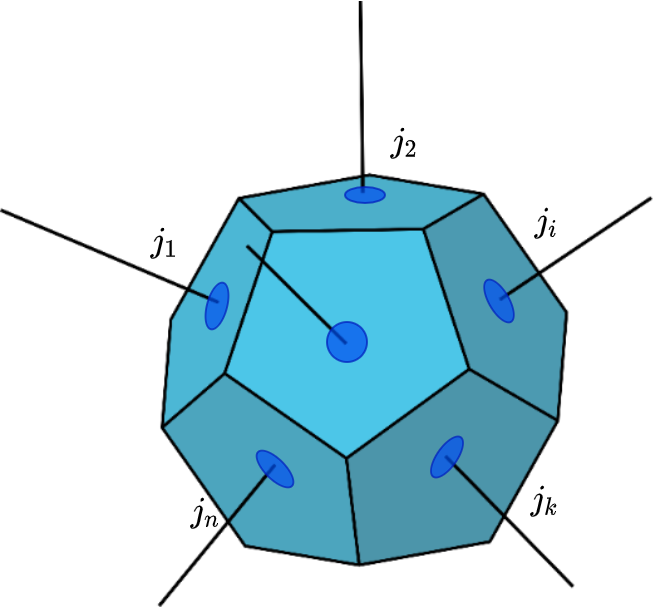
\includegraphics[width=0.5\linewidth]{polyhedron-spins.png}
	\caption{An example of a spin-network vertex, with the associated polyhedron. The faces of the polyhedron are transverse to the edges attached to the vertex. The vertex itself lies in the interior of the polyhedron. Each edge punctures one of the faces and assigns it a quantum of area depending on the spin rep labelling the edge.}
	\label{fig:polyhedron-spins}
\end{figure}


\subsection{Spinorial LQG}\label{sec:spinorial-lqg}

The spinorial formulation of LQG was developed in a series of seminal papers by Freidel and Speziale \cite{Freidel2010Twisted,Freidel2010From}. The classical phase space of a single spin network edge is given by $ T^*[SU(2)] \simeq SU(2) \times \mf{su}(2) $ - the cotangent bundle on $ SU(2) $. Configuration variables are group elements $ g \in SU(2)$ and the momenta are elements of the lie algebra $ \mf{su}(2) $. Recall that the Hilbert space of a \textit{single} edge is given by \eqref{eqn:edge-hilbert-space} the space of square integrable functions $ \mc{L}^2[SU(2)] $ on $ SU(2) $. This space can be viewed as the quantization of the classical phase space $ T^*[SU(2)] $.

\begin{figure}
	\centering
	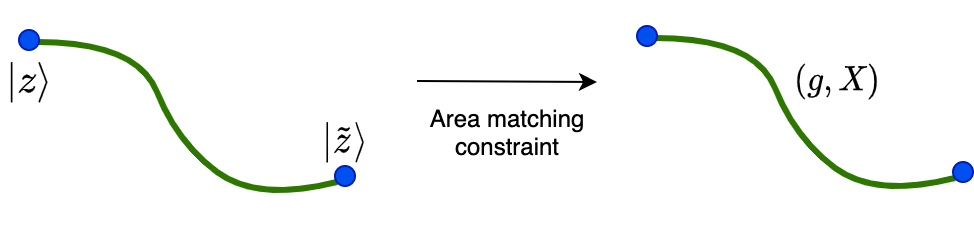
\includegraphics[width=\linewidth]{spinorial-lqg}
	\caption{In spinorial LQG we label each end of an edge with spinors $ (\ket{z}, \ket{\tilde z}) \in \C^2 \times \C^2$. Applying the area matching constraint $ \norm{z}^2 - \norm{\tilde z}^2 = 0 $, we obtain the phase space variables $ (g,X) $, with $ g \in SU(2) $ and $ X \in \mf{su}(2) $.}
	\label{fig:spinorial-lqg}
\end{figure}

What was shown in the works by Freidel and Speziale was that one can obtain $ T^*[SU(2)] $ by starting from the space $ \C^2 \times \C^2 $ whose elements are pairs of spinors $ \ket{z}, \ket{\tilde z} $. From each spinor we can construct a three-vector as follows:
\begin{equation}\label{eqn:spinors-to-face-normal}
	\vec{X} = \expectop{z}{\vec{\sigma}}{z}; \quad \vec{\tilde X} = \expectop{\tilde z}{\vec{\sigma}}{\tilde z}
\end{equation}
where $ \vec{\sigma} = (\sigma_x, \sigma_y, \sigma_z)$ are the three Pauli matrices. For a brief introduction to spinorial notation we refer the reader to Appendix \ref{sec:spinor-notation}. These vectors are then to be thought as corresponding to the normals to the faces which are dual to a given edge (\autoref{fig:spinor-normals}). In the classical picture, the area of a face is given by the length of the vector normal to it. Thus, the vectors $ \vec{X}, \vec{\tilde X} $ are the classical counterparts of the angular momentum operators $ \vec{J} $ assigned to each end of an edge. These vectors satisfy the identity:
\begin{equation}\label{eqn:vector-norm}
	\norm{X} = \innerp{z}{z}; \quad \norm{\tilde X} = \innerp{\tilde z}{\tilde z}
\end{equation}
We can construct the momentum variable - the element of $ \mf{su}(2) $ - associated with each end of a vertex by taking the corresponding face normals and contracting them with the Pauli matrices:
\begin{equation}\label{eqn:momentum-variables}
	X = \vec{X} \cdot \vec(\sigma); \quad \tilde X = \vec{\tilde X} \cdot \vec{\sigma}
\end{equation}

We can construct the group element $ g \in SU(2) $ corresponding to the holonomy along the given edge (and plays the role of the configuration variable of the classical phase space $ T^*[SU(2)] $) as follows:
\begin{equation}\label{eqn:spinors-to-holonomy}
	g(z,\tilde z) = \frac{\ket{z}\rbra{\tilde z} - \rket{z}\bra{\tilde z}}{\norm{z} \norm{\tilde z}}
\end{equation}

\begin{figure}[htbp]
	\centering
	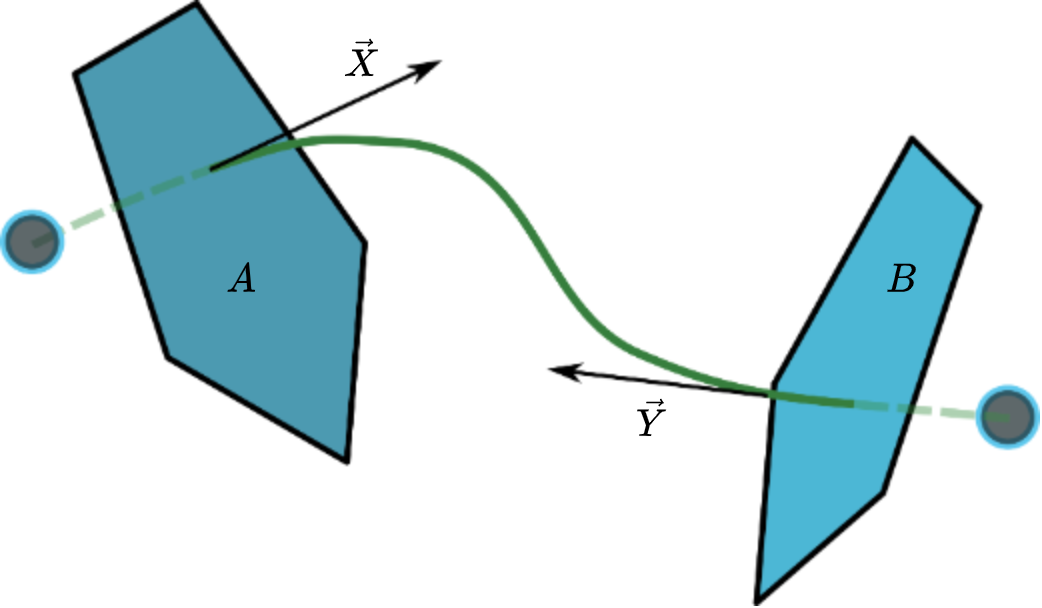
\includegraphics[width=0.8\linewidth]{spinor-normals-labelled}
	\caption{The normal vectors to the faces at each end of an edge in terms of the spinors attached to each end.}
	\label{fig:spinor-normals}
\end{figure}

Now, in order for the spin network to correspond to a triangulation of our background manifold, we must be able to glue the faces labelled $ A $ and $ B $ in \autoref{fig:spinor-normals} to each other. This implies the area of the two faces must match. Since the area of a face is proportional to the length of the face normal, this implies the following \textit{area matching constraint} on the two spinors $ \ket{z} $ and $ \ket{\tilde z} $:
\begin{equation}\label{eqn:area-matching}
	\mc{M} = \innerp{z}{z} - \innerp{\tilde z}{\tilde z} = 0,
\end{equation}
must hold. It is the imposition of this constraint which allows us to reduce the spinorial phase space $ \C^2 \times \C^2 $ to the phase space of a single edge $ T^*[SU(2)] $.

In \cite{Freidel2010From,Freidel2010Twisted} the authors showed the following correspondence:
\begin{equation}\label{eqn:symplectic-reduction}
	T^*[SU(2)] \simeq (\C^2 \times \C^2)//U(1),
\end{equation}
where the ``double quotient'' is understood as taking those elements of $ \C^2 \times \C^2 $ which live on the constraint surface determined by \eqref{eqn:area-matching} and which Poisson commute with this constraint. It is understood that degenerate points, \ie those for which $ \norm{X} = 0 $, $ \innerp{z}{z} = 0 $, $ \innerp{\tilde z}{\tilde z} = 0 $ are excluded from both sides of the above relation.

We can now address what we set out to do - labeling the classical phase space of the intertwiner. For this purpose we simply need to label the ends of intertwiner legs which meet the given vertex with spinor $ \ket{z_i}; i \in \{1,\ldots,n\} $ as shown in \autoref{fig:polyhedron-spinors}.

\begin{figure}[htbp]
	\centering
	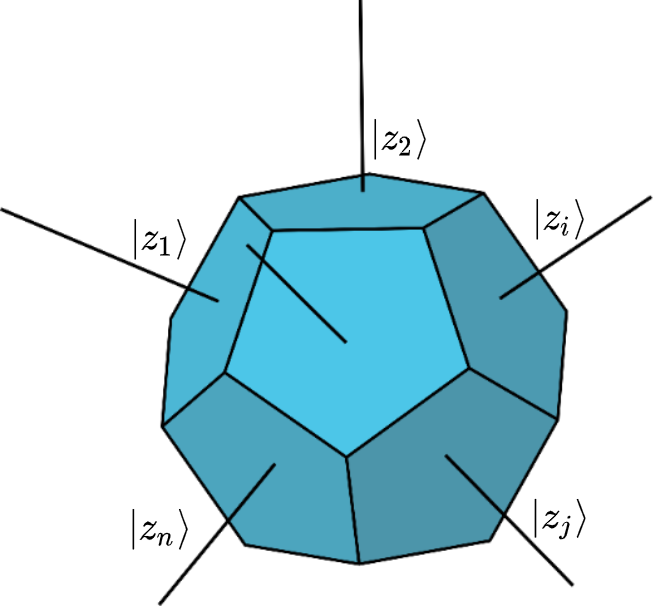
\includegraphics[width=0.5\linewidth]{polyhedron-spinors}
	\caption{The classical phase space of an intertwiner. Each leg is labelled by a spinor $ \ket{z_i} \in \C^2 $ where $ i \in \{1,\ldots,n\} $.}
	\label{fig:polyhedron-spinors}
\end{figure}
It is this set of spinors which provides us with the set of labels needed to parametrize a given $ U(N) $ coherent state.

\subsection{$ U(n) $ Coherent Intertwiners}\label{sec:u-n-thermal-coherent-states}

In order to construct coherent states for intertwiners we first use the Schwinger boson trick to write the spin associated with each face in terms of two oscillators. This step is illustrated in the lower half of \autoref{fig:schwinger-boson-rep}. There both of the spins at \textit{both} ends of a given edge are mapped to their respective pair of oscillators. In our case we our only interested in a single quantum of spacetime volume which corresponds to a single $ n $-valent single vertex, so we only care about what happens at \textit{one} end of an edge which meets a given face of that intertwiner. The end result is illustrated in \autoref{fig:polyhedron-bosons}.

\begin{figure}
	\centering
	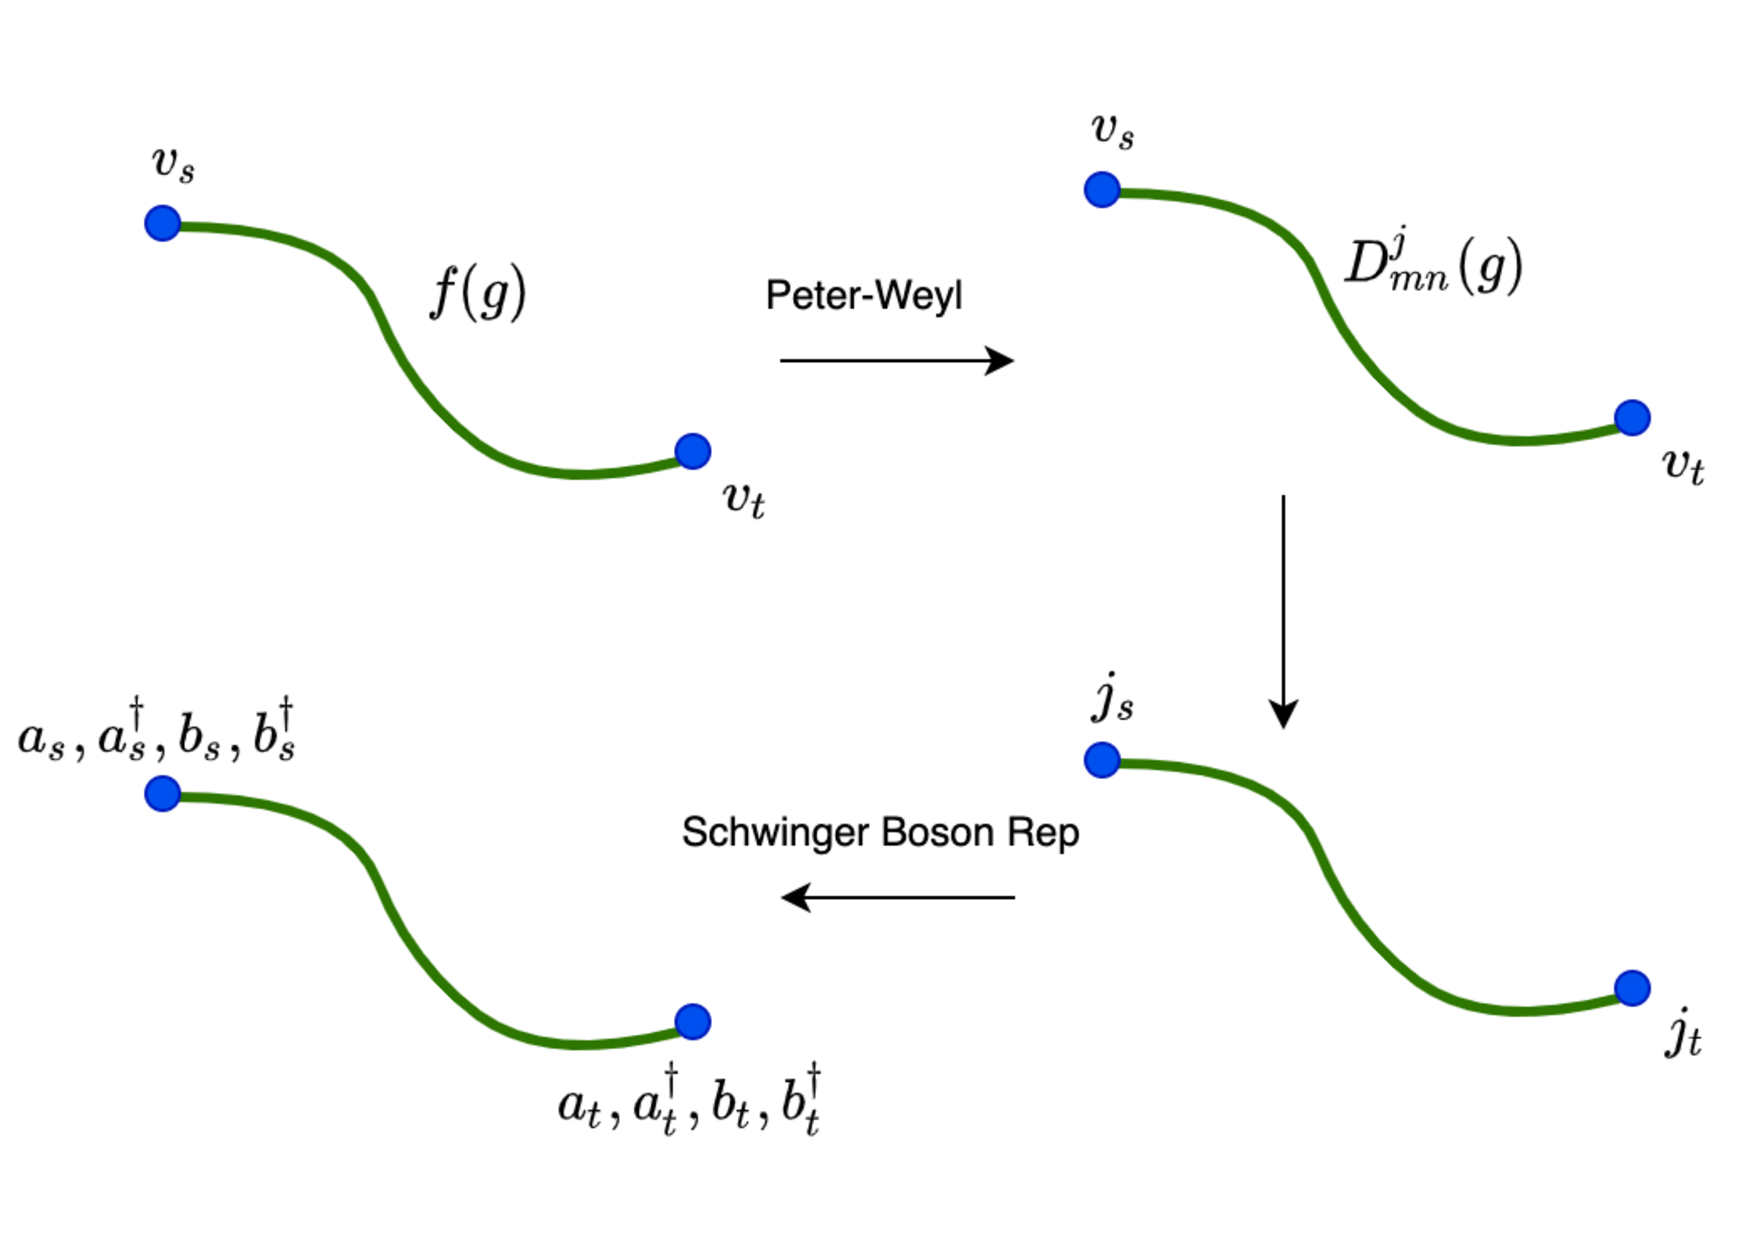
\includegraphics[width=\linewidth]{schwinger-boson-edge.pdf}
	\caption{Illustration of steps leading from cylindrical functions of edge holonomies to Schwinger Boson basis with pairs of ladder operators assigned to the source and target vertices respectively.}
	\label{fig:schwinger-boson-rep}
\end{figure}

We now define the following operators which act on \textit{pairs} of faces:
\begin{equation}\label{eqn:u-n-generators}
	E_{ij} = a_i^\dagger a_j + b^\dagger_i b_j.
\end{equation}
These operators have a very simple physical interpretation. They destroy one quantum of type $ a $ and of one of type $ b $ living the $ j $\supersc{th} face and create one quantum of type $ a $ and one of type $ b $ on the $ i $\supersc{th} face. We can think of operator as a \textit{hopping} term in the language of many body physics. It is clear that this operator is hermitian. What makes these operators useful is that they commute with the generator of global $ SU(2) $ transformations generated by the \textit{total} angular momentum operator $ \vec{J} = \sum_{i=1}^n \vec J_i $:
\begin{equation}\label{eqn:e-j-commutator}
	\left[\vec{J}, E_{ij} \right] = 0 \quad \forall i,j.
\end{equation}
Furthermore the set of operators $ E_{ij} $ with $ i,j \in \{1,2,\ldots,n\} $ is closed under commutation \cite{Freidel2010UN-Coherent}:
\begin{equation}\label{eqn:u-n-algebra}
	[E_{ij}, E_{kl}] = \delta_{jk} E_{il} - \delta_{il} E_{kj},
\end{equation}
which we recognize to be the Lie algebra of the group $ U(n) $. If we choose to measure the area of a face with the Freidel-Livine prescription \eqref{eqn:freidel-livine} rather than the Rovelli-Smolin prescription \eqref{eqn:rovelli-smolin}, then from \eqref{eqn:schwinger-energy-op} we see that for $ i=j $, the operator $ E_i \equiv E_{ii} $ corresponds to \textit{twice} the area of the $ i $\supersc{th} face. The operator $ E = \sum_{i=1}^{n} E_i $ therefore corresponds to \textit{twice} the total area of the polyhedron. The operators $ E_{ij} $ generate $ U(n) $ transformations of the polyhedron which correspond to \textit{area-preserving} diffeomorphisms. This property can be seen by noting that the action of $ E_{ij} $ on the $ j $\supersc{th} face lowers $ j_j $ by $ 1/2 $ and its action on the $ i $\supersc{th} face raises the value of $ j_i $ by $ 1/2 $, thus keeping the sum $ \sum_{i=1}^{n} j_n $, which corresponds to the total area, a constant.

In order to define $ U(n) $ coherent states we need one more ingredient. These are the $ U(n) $ ladder operators given by:
\begin{equation}\label{eqn:u-n-ladder-ops}
	F_{ij} = a_i b_j - a_j b_i; \quad F^\dagger_{ij} = a^\dagger_i b^\dagger_j - a^\dagger_j b^\dagger_i.
\end{equation}
We define $ \bket{0} $ to be the Fock vacuum, which satisfies $ F_{ij} \bket{0} = 0,~\forall i,j $. We can now define the $ U(n) $ coherent states:
\begin{equation}\label{eqn:u-n-coherent-states}
	\bket{J, z_i} = \frac{1}{\sqrt{J+1}}\frac{(F^\dag_\bz)^J}{J!}\bket{0}.
\end{equation}
Here $ J $ measures the total area of the coherent polyhedron represented by this state; and $ \bz \equiv z_{ij} $ is a matrix defined in terms of $ \{z_i\} $ which are the spinor labels assigned to the end of each edge adjacent to the given vertex as shown in \autoref{fig:polyhedron-spinors}. As explained in the previous section, these spinors label a point in the classical phase space of $ n $ sided polyhedra. Using these spinors we define:
\begin{equation}\label{eqn:spinor-matrix}
	\bz \equiv z_{ij} = \innerpB{z_i}{z_j}
\end{equation}
where the inner product in the above expression is defined in \eqref{eqn:spinor-bilinears}. Using the definition of $ z_{ij} $ one can show that $ z_{ij} = - z_{ji} $, i.e. that $ \bz $ is an anti-symmetric matrix. The quantity $ F^\dag_\bz $ in \eqref{eqn:u-n-coherent-states} is defined as follows:
\begin{equation}\label{eqn:ladder-ops-v2}
	F_\bz = \onehalf \sum_{ij} \bar z_{ji} F_{ij}; \quad F^\dag_\bz = \onehalf \sum_{ij} z_{ji} F^\dag_{ij}.
\end{equation}

\begin{figure}
	\centering
	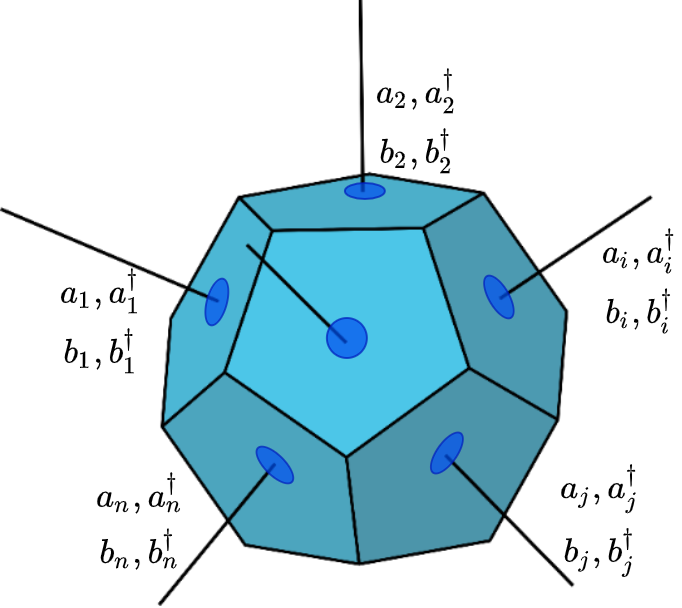
\includegraphics[width=0.5\linewidth]{polyhedron-bosons.png}
	\caption{Applying the Schwinger boson trick to each spin label on all the edges.}
	\label{fig:polyhedron-bosons}
\end{figure}

In the definition of these coherent state \eqref{eqn:u-n-coherent-states} there is a parameter $ J $. One can see that this parameter corresponds to the total area of the $ n $ sided polyhedron as follows. A straightforward computation shows that:
\begin{equation}\label{eqn:e-f-commutator}
	[E, F^\dag_\bz] = 2 F^\dag_\bz
\end{equation}
where $ E = \sum_i E_i $; and $ E_i := E_{ii} $ are the diagonal generators of the $ \mf{u}(n) $ algebra. Using this expression along with standard commutator identities one can show that:
\begin{equation}\label{eqn:e-f-commutator-v2}
	[E, (F^\dag_\bz)^J] = 2 J (F^\dag_\bz)^J; \quad \forall J \in \mathbb{N}.
\end{equation}
Applying this expression to the definition of the coherent states \eqref{eqn:u-n-coherent-states} one can show that:
\begin{equation}\label{eqn:e-eigenvalue}
	E \bket{J, z_i} = 2 J \bket{J, z_i}
\end{equation}
From the discussion following \eqref{eqn:u-n-algebra} we know that eigenvalues of the operator $ E $ correspond to \textit{twice} the area of the polyhedron. Therefore we can identify $ J $ in the above expressions as the total area of the polyhedron.

It can be shown explicitly \cite{Freidel2010UN-Coherent} that these states \eqref{eqn:u-n-coherent-states} are indeed generalized coherent states in the sense of Perelomov \cite{Perelomov1977Generalized} and are generated by the action of elements of $ U(n) $ on the highest weight vector. As a result they are also minimum uncertainty states in that the following ratio: $ \Delta E_{ij}/\expect{E_{ij}} \sim 1/\sqrt{J} $ vanishes in the limit of large values for the total area $ A_{tot} = 2 J  $ of the polyhedron. Here:
\begin{equation}\label{eqn:e-op-uncertainty}
	\Delta^2 E_{ij} = \expect{E_{ij}E_{ji}} - \expect{E_{ij}} \expect{E_{ji}}
\end{equation}
is the dispersion in the expectation value of the operators $ E_{ij} $.

\section{Coherent Thermal Intertwiners}\label{sec:thermal-intertwiners}

We now have all the ingredients in hand in order to construct \textit{thermal} $ U(n) $ coherent intertwiners. One might think that the procedure to do would be the following:
\begin{enumerate}[label=\emph{\alph*})]
	\item construct the thermalizing operator $ U(\beta) $ \eqref{eqn:u-beta}
	\item use $ U(\beta) $ to obtain the thermalizing ladder operators as shown in \eqref{eqn:thermal-ladder-ops}
	\item use these thermalized ladder operators to construct the coherent thermal state.
\end{enumerate}
However, there are some subtleties along the way we have to take care of. The first is the following. The construction of the $ \mf{su}(2) $ coherent thermal states \eqref{eqn:su2-thermal-coherent-state} double state described in \autoref{sec:tfd-state} requires a pair of oscillators. We already have these in the form of the oscillator pairs $ a_i, b_i $ assigned to each face of the polyhedron. However, now rather than just one spin we now have to define the thermal coherent state of $ n $ spins. This would suggest that rather than a single inverse temperature $ \beta $ we now need $ n $ different values of the inverse temperature $ \beta_i $, one for each face of the polyhedron. We could proceed by assuming that each face is at a different temperature and construct the global thermalizing operator:
\begin{equation}\label{eqn:global-u-beta}
	\mb{U} = U(\beta_1) \otimes U(\beta_2) \otimes \ldots \otimes U(\beta_n),
\end{equation}
where $ U(\beta_i) $ is the thermalizing operator acting on the Hilbert space of the $ i $\supersc{th} puncture. It is straightforward to see that the closure constraint \eqref{eqn:gauss-constraint} remains unchanged under the action of this global $ \mb{U} $:
\begin{equation}\label{eqn:closure-preserved}
	\sum_{i=1}^{n} \vec{J}_i = 0 \Rightarrow \mb{U} \left( \sum_{i=1}^{n} \vec{J}_i \right) \mb{U}^{-1} = 0
\end{equation}
%This by itself is not sufficient to ensure that the thermal intertwiner state constructed using $ \mb{U} $ will correspond to the state of a coherent polyhedron. 
It is not sufficient to understand only how the individual face Hilbert space transform under the thermalizing operator because this is not a system of $ n $ \textit{independent} spins. Rather the coherent state constructed via \eqref{eqn:u-n-coherent-states} relies on the operators $ F_{ij} $ which link pairs of different faces and do not transform in a simple manner under $ U_{ij} = U(\beta_i) \otimes U(\beta_j) $.

We can circumvent these issues by making the assumption that the inverse temperature $ \beta_i = \beta $ is the same for all faces. In this case the operators $ E_{ij} $ and $ F_{ij} $ \textit{will} have a simple transformation under the global $ \mb{U} $ and one can verify that the thermalized $ E_{ij}(\beta) $ will continue to satisfy the $ U(n) $ Lie algebra given in \eqref{eqn:u-n-algebra}. The assumption of having the same temperature for all faces is not just a mathematical convenience. It has a deep physical significance. In the context of black hole thermodynamics, for instance, this condition would correspond to the assumption of equipartition of energy between the microstates which constitute the horizon macrostate for a given value of the area $ A $.

By assuming same temperature for all the surfaces, the expression for $ \mb{U}$ is given as
\begin{equation}
	\mb{U} = exp\left[\sum_{i=1}^{N}\theta[ a_{i_{L}}^{\dagger} a_{i_{R}}^{\dagger} - \ a_{i_{L}} a_{i_{R}} + b_{i_{L}}^{\dagger} b_{i_{R}}^{\dagger} - b_{i_{L}} b_{i_{R}}]\right]
\end{equation}

The final expression for thermal coherent states for a semiclassical geometry corresponding to a $ n $-valent polyhedron is therefore given by:
\begin{equation}\label{eqn:u-n-thermal-coherent-state}
	\bket{J, z_i}_{\beta _{L}} = \frac{1}{\sqrt{J+1}}\frac{(\tilde F^\dag_{\bz _{L}})^J}{J!}\bket{0(\beta)},
\end{equation}
where $ \tilde F^\dag_\bz $ is defined in terms of the thermalized $ U(n) $ ladder operators:
\begin{equation}\label{eqn:u-n-thermal-ops}
	\tilde F_{ij} = a_i(\beta) b_j (\beta) - a_j(\beta) b_i(\beta)
\end{equation}
By operating with the $\tilde F^\dag_{\bz _{L}}$, we ensure that the $ 2^{nd}$ hilbert space $H_{R}$ remains at vacuum which means that the state $\bket{J, z_i}_{\beta}$ represents the thermal coherent states of the $ 1^{st}$ system.

From \eqref{eqn:thermal vacuum} and \eqref{eqn:thermal-ladder-ops}, we see that there is a clear connection between the 2 hilbert spaces which is induced by the temperature. In case of coherent intertwiners, these states represent the geometry and hence the temperature paramater connects the two geometries which basically is a description of wormhole geometry. Thus the finite temperature state of an extended Hilbert Space gives a mathematical description of wormhole geometry. 
\section{Discussion: }\label{sec:discussion}



\begin{acknowledgements}
	DV thanks the Inter-University Center for Astronomy and Astrophysics (IUCAA), Pune for support under the Visiting Associates program. The authors would also like to thank their respective families for continuing support and inspiration.
\end{acknowledgements}

\appendix

\section{Derivation of Thermofield Double State}\label{sec:tfd}

The material in this section is standard and is included here to make the article self-contained for most authors. We follow \cite[Sec 5.1]{Khanna2009Thermal} in the following. We want to find a thermal state $ \ket{0(\beta)} $ which satisfies the following condition: \textit{the expectation value of any operator in $ \ket{0(\beta)} $ is identical to the statistical ensemble average of the matrix elements of that operator}. This can be written as:
\begin{equation}\label{eqn:tfd-condition}
	\expect{A} = \expectop{0(\beta)}{A}{0(\beta)} = \frac{1}{Z} \sum_n e^{-\beta E_n} \expectop{n}{A}{n}
\end{equation}
To proceed, let us assume that $ \ket{0(\beta)} $ is a vector in the original Hilbert space $ \mc{H}_0 $ whose basis is given by the states $ \{ \ket{n}, n \in \mbb{Z} \} $, in which case $ \ket{0(\beta)} $ can be expanded in this basis:
\begin{equation}\label{eqn:tfd-expansion}
	\ket{0(\beta)} = \sum_n c_n \ket{n} \nonumber
\end{equation}
Substituting this expression back in \eqref{eqn:tfd-condition} we find:
\begin{equation}
	\expectop{0(\beta)}{A}{0(\beta)} = \sum_{m,n} c^*_m c_n \expectop{m}{A}{n} = \frac{1}{Z} \sum_n e^{-\beta E_n} \expectop{n}{A}{n} \nonumber
\end{equation}
The second equality on the right will hold if the coefficients $ c_n $ satisfy an orthogonality condition:
\begin{equation}\label{eqn:ortho-condition}
	c^*_m c_n = \frac{1}{Z} \sum_n e^{-\beta E_n} \delta_{mn}
\end{equation}
However, such a condition cannot be satisfied if the coefficients $ c_n $ are scalars ($ \C $ numbers in this case). This implies that the state $ \ket{0(\beta)} $ cannot be an element of the original state space $ \mc{H}_0 $. The above condition \textit{would} be satisfied in the coefficients $ c_n $ were vectors instead of scalars. Though one could take the representative set of vectors to be any orthogonal basis of $ \mc{H}_0 $, it turns out to be simplest to identify the $ c_n $ with elements of the energy eigenbasis:
\begin{equation}
	c_n \rarrow \ket{c_n} = d_n(\beta) \ket{n} \nonumber
\end{equation}
Inserting this expression into \eqref{eqn:tfd-expansion} we see that the state $ \ket{0(\beta)} $ can be written as:
\begin{equation}\label{eqn:tfd-state2}
	\ket{0(\beta)} = \sum_n d_n(\beta) \ket{n} \ket{\tilde n} \nonumber
\end{equation}
This is no longer a state in the Hilbert space $ \mc H_0 $ we started with, but in the ``double copy'' $ \mc{H} = \mc{H}_0 \otimes \mc{H}_0 $ space. We have put a $ \tilde{} $ over the second occurrence of $ n $ to indicate that it refers to states in the second copy of the Hilbert space.  Since the thermofield double does not live in the same Hilbert space as the original system, the natural question is how can one calculate thermal expectation values for operators which act on the original system using the thermofield state? We can do this as follows. Given any operator $ \hat A $ which acts on $ \mc{H}_0 $, we can extend this to an operator $ \hat {\mc A} $ which acts on $ \mc{H} $, via:
\begin{equation}\label{eqn:operator-extension}
	\hat A \rarrow \hat {\mc A} = \hat A \otimes \id.
\end{equation}
If we now evaluate the expectation value of $ \hat {\mc A} $ on the state $ \ket{0(\beta)} $ defined in \eqref{eqn:tfd-state2} we find:
\begin{align}
	\expectop{0(\beta)}{\hat{\mc A}}{0(\beta)} & = \sum_{m,n} d^*_m(\beta) d_n(\beta)\expectop{m}{\hat A}{n} \innerp{\tilde m}{\tilde n} \nonumber \\
	&= \sum_n |d_n(\beta)|^2 \expectop{n}{\hat A}{n}
\end{align}
Note that, as before, $ \tilde m $ and $ \tilde n $ are numerically equal to $ m $ and $ n $. Requiring the above expression to match the r.h.s of \eqref{eqn:tfd-condition} implies that the coefficients are given by:
\begin{align}
	d_n(\beta) = \frac{e^{-\beta E_n/2}}{\sqrt{Z}}, \nonumber
\end{align}
which brings us to our final expression for the thermofield double state for a harmonic oscillator at an inverse temperature $ \beta $:
\begin{align}
	\ket{0(\beta)} = \frac{1}{\sqrt{Z}} \sum_n  e^{-\beta E_n/2} \ket{n,\tilde n} 
\end{align}

\section{Unitary Operator for Thermal States}\label{sec:thermal-unitary}

Recalling that the number operator states can be written in terms of the action of ladder operators \eqref{eqn:ladder-ops} on the vacuum $ \ket{0} $, the thermofield state can be written as:
\begin{align}
	\ket{0(\beta)} & = \frac{1}{\sqrt{Z}} \sum_n e^{-\beta E_n/2} \frac{(a_L^\dagger)^n}{\sqrt{n!}} \frac{(a_R^\dagger)^n}{\sqrt{n!}} \ket{0,\tilde 0} \nonumber \\
	& = \frac{1}{\sqrt{Z}} \sum_n \frac{\left( e^{-\beta \hbar \omega/2} a_L^\dagger a_R^\dagger \right)^n}{n!} \ket{0,\tilde 0} \nonumber \\
	& = \frac{1}{\sqrt{Z}} \exp{\left(e^{-\beta \hbar \omega/2} a_L^\dagger a_R^\dagger \right) } \ket{0,\tilde 0},
\end{align}
where in the second line we have used the fact that for a harmonic oscillator the energy eigenvalues are given by $ E_n = n \hbar \omega $. In the final step we note that the sum over the coefficients in the second step is the Taylor series expansion of the exponential of an operator $ e^{-\beta \hbar \omega/2} a_L^\dagger a_R^\dagger $. In fact one can show (see \eg, \cite[Sec 6]{Khanna2009Thermal}) that the thermal state can be obtained from the doubled copy ground state by the action of a unitary operator:
\begin{equation}\label{eqn:unitary-op-action}
	\ket{0(\beta)} = e^{-i G(\theta)} \ket{0,\tilde 0}
\end{equation}
where the operator $ G(\theta) $ is given by:
\begin{equation}\label{eqn:unitary-op-generator}
	G(\theta) = -i \theta(\beta) (a_L a_R - a_L^\dagger a_R^\dagger).
\end{equation}
Here $ \theta(\beta) $ is related to the inverse temperature $ \beta $ by:
\begin{equation}\label{eqn:temp-theta-relation}
	\theta(\beta) = \tanh^{-1}(e^{-\beta \hbar \omega/2})
\end{equation}
It can be easily seen that $ G(\theta) $ is a Hermitian operator and therefore $ e^{-iG(\theta)} $ is a unitary operator.

\section{Spin Coherent State Projection}\label{sec:spin-projection}

In order to implement the constraint $ 2j = n_a + n_b $ in \eqref{eqn:pair-coherent-state} we first rewrite that expression as a sum over $ j,m $ instead of a sum over $ n_a, n_b $:
\begin{align}
	& \ket{z_a, z_b} = e^{-(|z_a|^2 + |z_b|^2)/2} \sum_{n_a, n_b} \frac{z_a^{n_a} z_b^{n_b}}{\sqrt{n_a! n_b!}} \ket{n_a, n_b} \nonumber \\
 	& = e^{-(|z_a|^2 + |z_b|^2)/2} \sum_{j=0}^{\infty} \sum_{m=-j}^{j} \frac{z_a^{j+m} z_b^{j-m}}{\sqrt{(j+m)! (j-m)!}} \ket{j, m} \nonumber \\
	& = e^{-(|z_a|^2 + |z_b|^2)/2} \sum_{j=0}^{\infty} z_a^j z_b^j \sum_{m=-j}^{j} \frac{z_a^m z_b^{-m}}{\sqrt{(j+m)! (j-m)!}} \ket{j, m},
\end{align}
where in the second line we have simply rewritten the sum over $ n_a, n_b $ as being over $ j,m $ and in the next step we have pulled out factors of $ z_a, z_b $ which depend on $ j $. Now define $ z = z_b/z_a $. This implies $ z_b = z z_a $ and:
\begin{equation*}
	z_a^{j+m} z_b^{j-m} = z_a^{j+m} z^{j-m} z_a^{j-m} = z_a^{2j} z^{j-m}
\end{equation*}
Using this the we can write the projected spin coherent state as:
\begin{equation}
	P_j \ket{z_a, z_b} = e^{-(|z_a|^2 + |z_b|^2)/2} z_a^{2j} \ket{j;z},
\end{equation}
where $ \ket{j;z} $ is given by:
\begin{equation}
	\ket{j;z} = \sum_{m=-j}^{j} \frac{z^{j-m}}{\sqrt{(j+m)! (j-m)!}} \ket{j;m}.
\end{equation}

\section{LQG Phase Space}\label{sec:lqg-phase-space}

The Hilbert space consists of cylindrical functions $ \psi(h_1, \ldots, h_{N_e}) $ where $ h_1, \ldots, h_{N_e} $ are $ SU(2) $ valued holonomies of the Ashtekar-Barbero connection along each edge. The (kinematic) Hilbert space of a graph thus consists square integrable functions on $ N_e $ copies of $ SU(2) $:
\begin{equation}\label{eqn:lqg-hilbert-1}
	\mc H_\Gamma = \mc L^2(SU(2)^{N_e})
\end{equation}

We can use the Peter-Weyl theorem to write functions on $ SU(2) $ in terms of spin labels (representations of $ SU(2) $) living on each edge:
\begin{equation}\label{eqn:peter-weyl}
	\psi(g) = \sum_{j;mn} f^{mn}_j D^j_{mn}(g)
\end{equation}
where $ \psi(g):SU(2) \rightarrow \C $ is a function of the holonomy, $ j $ labels the different irreps of $ SU(2) $, $ D^j_{mn} $ are the matrix elements of the group element $ g $ in the irrep $ j $ and $ f^{mn}_j $ are the coefficients of the function in the spin basis. Now each matrix $ D^j $ is $ (2j+1) \times (2j+1) $ matrix and therefore can be viewed as a map from one copy of $ \mc{H}_j $ to another copy:
\begin{equation}\label{eqn:irrep-map}
	D^j : \mc{H}_j \rightarrow \mc{H}_j
\end{equation}
Alternatively $ D^j $ can also be viewed as an element of $ \mc{H} \otimes \mc{H} $. Therefore the space of square-integrable functions on $ SU(2) $ can be written in terms of a direct sum of all irreps of two copies of $ SU(2) $:
\begin{equation}\label{eqn:edge-hilbert-space}
	\mc{L}^2(SU(2)) = \oplus_j (\mc{H} \otimes \mc{H})
\end{equation}
This is what leads us to what will be the most crucial point going forwards: \textit{with each edge there are associated two copies of the Hilbert space of a spin $ j $ particle}. This is shown in the upper half \autoref{fig:schwinger-boson-rep}.

\section{Spinor Notation}\label{sec:spinor-notation}

In this section we present some basic notations and relations involving spinors \cite{Livine2011Loop} which are required for understanding some of the expressions in the main text. A spinor $ \ket{z} $ is an element of $ \C^2 $, while $ \bra{z} $ is its hermitian adjoint:
\begin{equation}\label{eqn:spinors}
	\ket{z} = \begin{pmatrix}
		z^0 \\ z^1
	\end{pmatrix}; \quad \bra{z} = \begin{pmatrix}
									\bar z^0 & \bar z^1
									\end{pmatrix}
\end{equation}
The ``dual spinor'' $ \rket{z} $ is defined in terms of the spinor $ \ket{z} $ as follows:
\begin{equation}\label{eqn:dual-spinors}
	\rket{z} = \epsilon \rket{\bar z} = \begin{pmatrix}
											-\bar z^1 \\ \bar z^0
										\end{pmatrix}
\end{equation}
where $ \epsilon $ is the antisymmetric tensor with components:
\begin{equation}\label{eqn:epsilon-tensor}
	\epsilon = \begin{pmatrix}
					0 & -1 \\
					1 & 0
				\end{pmatrix}
\end{equation}
The combination of complex conjugation $ \ket{z} \rightarrow K \ket{z} = \ket{\bar z} $ followed by multiplication by $ \epsilon $ can be written as the map: $ J = \epsilon K $ which satisfies $ J^2 = -\id $. There are two different spinor bilinears:
\begin{align}\label{eqn:spinor-bilinears}
	\innerp{x}{y} & = \rinnerp{y}{x} = \bar x^0 y^0 + \bar x^1 y^1; \nonumber \\
	\innerpB{x}{y} & = -\innerpB{y}{x} = x^0 y^1 - x^1 y^0
\end{align}
From any spinor $ \ket{z} $ one can construct a Hermitian matrix which can be expanded in terms of the $ (\id, \vec{\sigma}) $ basis as follows:
\begin{equation}\label{eqn:spinor-matrix}
	\ket{z}\bra{z} = \onehalf (\innerp{z}{z} \id + \vec{X} \cdot \vec{\sigma})
\end{equation}
where $ \vec{X} \in \mbb{R}^3$ and $ \norm{X} = \innerp{z}{z}$. The above map is not one-to-one because a $ U(1) $ rotation $ \ket{z} \rightarrow e^{i\theta} \ket{z}$ leaves the matrix $ \ket{z}\bra{z} $, and hence the vector $ \vec{X} $, invariant. As mentioned in the text we can construct an element $ g \in SU(2) $ from two spinors via:
\begin{equation}
	g(z,\tilde z) = \frac{\ket{z}\rbra{\tilde z} - \rket{z}\bra{\tilde z}}{\norm{z} \norm{\tilde z}}
\end{equation}
The inverse of this element is equal to its Hermitian adjoint by unitarity of $ SU(2) $ and is given by:
\begin{equation}\label{eqn:holonomy-inverse}
	g^{-1}(z, \tilde z) = g^\dag(z, \tilde z) = \frac{\rket{\tilde z}\bra{z} - \ket{\tilde z}\rbra{z}}{\norm{z} \norm{\tilde z}}
\end{equation}
It is easy to verify using the spinor bilinear identities given in \eqref{eqn:spinor-bilinears} that indeed: $ g^{-1} g = \id $. It takes a little more work to verify that $ \det(g) = 1 $. The action of the holonomy on spinors (when the area matching constraint \eqref{eqn:area-matching} is satisfied) is given by:
\begin{equation}\label{eqn:holonomy-action}
	g \frac{\ket{\tilde z}}{\norm{\tilde z}} = -\frac{\rket{z}}{\norm{z}}; \quad g^{-1} \frac{\ket{z}}{\norm{z}} = \frac{\rket{\tilde z}}{\norm{\tilde z}}
\end{equation}
Using \eqref{eqn:spinors-to-holonomy} one can verify that under the \textit{local} action of $ SU(2) $ on a spinor pair:
\begin{equation}\label{eqn:su2-spinor-action}
	(\ket{z}, \ket{\tilde z}) \rightarrow (h_1 \ket{z}, h_2 \ket{\tilde z}),
\end{equation}
the holonomy $ g(z, \tilde z) $ transforms exactly as a holonomy should:
\begin{equation}\label{eqn:su2-holonomy-action}
	g(z, \tilde z) \rightarrow h_1 g(z, \tilde z) h_2^{-1},
\end{equation}
where $ h_1, h_2 \in SU(2) $ are gauge transformations acting on the source and target vertices of a given edge respectively. One can verify that when \eqref{eqn:area-matching} holds, the $ \mf{su}(2) $ element $ X = \vec{X}\cdot\vec{\sigma} $ (corresponding to $ \ket{z}) $ and the element $ \tilde{X} = \vec{\tilde X}\cdot\vec{\sigma} $ (corresponding to $ \ket{\tilde z} $) satisfy:
\begin{equation}\label{eqn:3-vecs-relation}
	\tilde X = -g^{-1} X g
\end{equation}

%\subsection{Reality Condition on Momenta}\label{sec:reality-condition}
%
%At this point the natural question to ask is what is the relation between the momenta of $ n $ massless particles as defined in \eqref{eqn:null-momenta} and the spinors labeling coherent intertwiners. Recall that in terms of a pair of spinors $ \lambda_\alpha, \tilde \lambda_{\dot \alpha} $ a momentum 4-vector can be expressed as:
%\begin{equation}\label{eqn:spinor-to-vector-1}
%	p_{\alpha \dot \alpha} = \lambda_\alpha \tilde \lambda_{\dot \alpha}	
%\end{equation}
%The requirement that $ p_{\alpha \dot \alpha} $ represent a real momentum reduces to the statement that:
%\begin{equation}\label{eqn:spinor-reality}
%	\tilde \lambda_{\dot \alpha} = \pm (\lambda^*_\alpha)	
%\end{equation}
%We choose the positive sign in this expression in order to select positive energy momenta.
%
%Given the spinor $ \ket{z} $ we can construct a future-pointing null 4-vector $ X^\mu = (X^0, X^i)$ whose components are given by \cite{Freidel2010From}:
%\begin{equation}\label{eqn:spinor-to-vector-2}
%	X^0 = \onehalf \innerp{z}{z}; \quad X^i = \expectop{z}{\vec \sigma}{z}
%\end{equation}
%The converse of the above equation becomes:
%\begin{equation}\label{eqn:vector-to-spinor-1}
%	\ket{z}\bra{z} = X^0 \id + X^i \sigma_i
%\end{equation}
%We can rewrite the above expression as:
%\begin{equation}\label{eqn:spinor-to-vector-3}
%	X_{\alpha \dot \alpha} = z_\alpha z^*_{\dot \alpha} \equiv (\ket{z}\bra{z})_{\alpha \dot \alpha}
%\end{equation}
%It is easy to see that the expression \eqref{eqn:spinor-to-vector-1} can be expressed in precisely the same manner due to the reality condition \eqref{eqn:spinor-reality}, as:
%\begin{equation}\label{eqn:spinor-to-vector-4}
%	p_{\alpha \dot \alpha} = \lambda_\alpha \lambda^*_{\dot \alpha} = (\ket{\lambda}\bra{\lambda})_{\alpha \dot \alpha}
%\end{equation}
%Thus the spinors $ \ket{z} $ used to label coherent intertwiners and the spinors $ \ket{\lambda} $ used to label massless particle momenta can be viewed as one and the same thing. To each edge of an intertwiner we can therefore assign a \textit{real}, null momentum 4-vector with components given by \eqref{eqn:spinor-to-vector-2} and in our interpretation this null vector is to be understood as representing the momentum of a massless particle.

%\bibliographystyle{naturemag}

%\bibliographystyle{h-physrev}

%\bibliographystyle{prsty}

\bibliographystyle{JHEP3}

%\bibliography{../bib_library.bib}

\bibliography{thermal-intertwiners.bib}

%\printbibliography

\end{document}

% arXiv leaks section

%As an aside let us address one source of doubt some readers might have at this point. The spin-statistics theorem tells us that particles with half-integer spin $ j \in \mbb{Z}/2 $ should obey fermionic statistics. However, in the Schwinger boson construction, as the name suggests, the oscillators in \eqref{eqn:sho-commutator} obey bosonic statistics. 

